\chapter{幾何、資訊與黑洞面積定律}

\lectureoverview{宣告的目的地是宇宙學，但通往那裡最短的路，得先回到狹義相對論。度規描述時空的幾何，而固有時為零的條件則描述光如何傳播。我們會把這條規則帶入施瓦西幾何，區分視界與奇點，再探問黑洞輻射殆盡後，資訊會如何。答案從一般的熵談起，最後落在貝肯斯坦的一位元論證：黑洞以視界面積而非體積為單位儲存資訊。}

蘇斯金德暫且擱下原本答應要談的弦理論成敗。他說，時間已晚，談實質內容比做一番盤點更有用。今晚要談的實質內容，是提出黑洞資訊問題所需的最低限度幾何與熱力學。

\section{光的一條規則}

狹義相對論把空間與時間視為同一個幾何對象。對於由\(dt,dx,dy,dz\)分隔的鄰近事件，蘇斯金德採用時間項為正的號差慣例，寫成
\begin{equation}
d\tau^2=dt^2-\frac{1}{c^2}\left(dx^2+dy^2+dz^2\right).
\end{equation}
時間項與空間項的符號相反，這使閔可夫斯基幾何有別於四維歐幾里得幾何。因子\(1/c^2\)只是用來調和單位；只要以一致的方式測量時間與距離，就可以令\(c=1\)。

對於類時分隔，\(d\tau^2>0\)，而\(d\tau\)是沿著該軌跡行進的時鐘所記錄的固有時。類空分隔則滿足\(d\tau^2<0\)。今晚要討論的情形恰好介於兩者之間。光線沿著\emph{零類}軌跡傳播，
\begin{equation}
d\tau^2=0.
\end{equation}
先限於沿\(x\)軸運動，可得
\begin{align}
0&=dt^2-\frac{dx^2}{c^2},\\
c\,dt&=\pm dx,\\
\frac{dx}{dt}&=\pm c.
\end{align}
正負號分別代表向右與向左傳播的光線。以\(c\)表示的數值會隨著單位從公分換成公尺或公里而改變；不變的陳述不是某個數值，而是零類條件。

廣義相對論改變的是度規的複雜程度，這條規則本身並沒有改變。以座標\(x^\mu\)、\(\mu=0,1,2,3\)表示，
\begin{equation}
ds^2=g_{\mu\nu}(x)\,dx^\mu dx^\nu,
\end{equation}
其中重複的指標代表求和，而係數可以隨位置改變。若要找出光在局部可行進的方向，就令這個二次型為零。

\section{球座標與施瓦西度規}

不旋轉的黑洞具有球對稱性，因此笛卡兒座標會掩蓋有用的結構。令\(r\)表示徑向距離，並以\(\theta,\phi\)標示單位球面上的方向。單位球面的線元素為
\begin{equation}
d\Omega^2=d\theta^2+\sin^2\theta\,d\phi^2.
\end{equation}
因此，在半徑為\(r\)的球面上，角位移所貢獻的項為\(r^2d\Omega^2\)。球座標中的平直時空則為
\begin{equation}
d\tau^2=dt^2-\left(dr^2+r^2d\Omega^2\right),
\qquad (c=1).
\end{equation}

蘇斯金德沒有從愛因斯坦方程推導黑洞解，而是直接寫出解，請我們仔細檢視。黑板清楚呈現了他要比較的內容。

\begin{figure}[htbp]
\centering
\includegraphics[width=0.86\textwidth]{lecture_02_figure_02.png}
\caption{施瓦西形變上方的平直球座標時空。重複出現的因子\(1-2GM/(c^2r)=1-R_s/r\)與徑向示意圖一同呈現。}
\lectureframe{00:19:12.520}
\end{figure}

對於質量為\(M\)的黑洞，施瓦西半徑定義為
\begin{equation}
R_s=\frac{2GM}{c^2}.
\end{equation}
外部區域的線元素為
\begin{equation}
d\tau^2=\left(1-\frac{R_s}{r}\right)dt^2
-\frac{dr^2/c^2}{1-R_s/r}
-\frac{r^2}{c^2}d\Omega^2.
\label{eq:schwarzschild-explicit-c}
\end{equation}
等價地，令\(c=1\)後，可寫成
\begin{equation}
ds^2=\left(1-\frac{2GM}{r}\right)dt^2
-\frac{dr^2}{1-2GM/r}-r^2d\Omega^2.
\label{eq:schwarzschild}
\end{equation}
在遠處，\(R_s/r\ll1\)，度規便回復為平直時空的球座標形式。這項漸近檢驗比背下公式更重要；不過蘇斯金德也建議把公式當作雞尾酒會上的談資。

\editorialnote{黑板上的寫法在\(d\tau^2\)與\(ds^2\)之間交替，而且\(c\)因子並未處處一致。方程~\eqref{eq:schwarzschild-explicit-c}採用講課中的時間座標慣例，其中\(t\)的單位是時間。使用\(x^0=ct\)的標準形式在代數上與之等價。}

\subsection{視界不是奇點}

在這套座標中，有兩個半徑看來值得懷疑。在自然單位制下，於\(r=R_s=2GM\)處，\(dt^2\)的係數為零，而\(dr^2\)的係數發散。在\(r=0\)處，曲率本身則變得奇異。這兩者並非同一事件的不同表現：
\begin{equation}
\begin{aligned}
r=R_s &:\quad \text{horizon},\\
r=0 &:\quad \text{curvature singularity}.
\end{aligned}
\end{equation}

潮汐力揭示了兩者在物理上的差別。引力場會在延展物體的不同位置有所變化：腳部受到的拉力可能比頭部更強，使身體受到拉伸，而橫向則受到擠壓。視界處的潮汐力有限；對質量足夠大的黑洞而言，視界處的潮汐力甚至可以很小，因此那裡不一定會發生任何局部災難。相較之下，\(r=0\)處的潮汐力會發散。\(r=R_s\)處令人警覺的係數顯示的是施瓦西座標的缺陷；\(r=0\)處的奇點則是物理上的奇點。

\editorialnote{可由克雷奇曼純量\(R_{\mu\nu\rho\sigma}R^{\mu\nu\rho\sigma}=48G^2M^2/(c^4r^6)\)檢查曲率在\(r=R_s\)處是否有限：該純量在視界處有限，只有當\(r\to0\)時才發散。講課中沒有寫出這個不變量，但它能精確表明潮汐力上的差異。}

\section{視界附近的徑向光線}

現在回到那條規則。徑向光線的角位置保持不變，因此\(d\Omega=0\)；而光線滿足\(ds^2=0\)。在\(c=1\)單位制下，方程~\eqref{eq:schwarzschild}給出
\begin{equation}
0=\left(1-\frac{2GM}{r}\right)dt^2
-\frac{dr^2}{1-2GM/r}.
\end{equation}
乘以\(1-2GM/r\)並開平方，可得兩個分支：
\begin{align}
dr&=\pm\left(1-\frac{2GM}{r}\right)dt,\\
\frac{dr}{dt}&=\pm\left(1-\frac{2GM}{r}\right).
\label{eq:radial-null}
\end{align}
正號代表向外傳播，負號代表向內傳播。在遠處，兩者的座標速度都趨近\(\pm1\)。在視界處，兩者都滿足\(\lvert dr/dt\rvert\to0\)：以施瓦西座標時間來看，向外傳播的光線似乎在那裡靜止，而向內傳播的光線則要經過無限長的座標時間才會抵達。

\begin{figure}[htbp]
\centering
\includegraphics[width=0.82\textwidth]{lecture_02_figure_03.png}
\caption{完成的\(t\)-\(r\)黑板示意圖：徑向零類光線愈接近虛線標示的視界，方向就愈趨近垂直。}
\lectureframe{00:30:25.000}
\end{figure}

\begin{figure}[htbp]
\centering
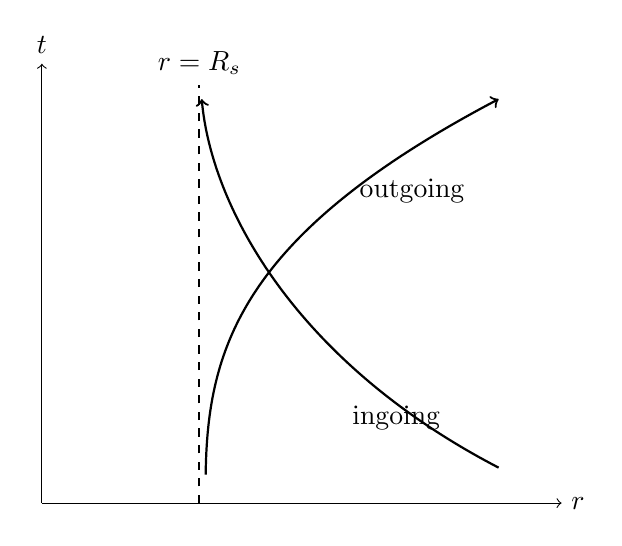
\begin{tikzpicture}[x=1.0cm,y=0.9cm]
\draw[->] (0,0) -- (6.6,0) node[right] {$r$};
\draw[->] (0,0) -- (0,6.2) node[above] {$t$};
\draw[dashed,thick] (2.0,0) -- (2.0,5.9) node[above] {$r=R_s$};
\draw[thick,->] (2.08,.4) .. controls (2.10,2.2) and (2.55,3.8) .. (5.8,5.7);
\draw[thick,->] (5.8,.5) .. controls (3.2,2.0) and (2.15,4.2) .. (2.03,5.7);
\node[align=center] at (4.7,4.4) {outgoing};
\node[align=center] at (4.5,1.2) {ingoing};
\end{tikzpicture}
\caption{黑板示意圖的座標時間版本，經過整理後如下。表觀上的減慢描述的是施瓦西座標\(t\)的性質，並不表示光在局部無法以\(c\)傳播。}
\end{figure}

在視界內，未來光錐向內傾斜得如此之大，以致兩個朝未來的徑向分支都指向\(r\)減小的方向。從那裡發出的訊號都無法逃到外部，而且每一條朝未來的因果路徑都會抵達奇點。

\begin{classroomqa}
\audiencequestion{如果光速是不變的，那麼說光在視界附近減慢，究竟是什麼意思？\lecturetimestamp{00:31:44}}
\lecturerresponse{這裡顯示的量\(dr/dt\)是特定座標系中的量。即使只是把公尺換成公分，速度的數值也會改變；在此處，有效的徑向與時間刻度會隨位置改變。普遍成立的陳述是，每條光線都沿零類軌跡傳播，\(ds^2=0\)。}
\end{classroomqa}
\editorialnote{自由落體的局部觀測者測得真空中的光速為\(c\)；視界處施瓦西座標速度趨於零，並非局部可觀測量。}

\begin{classroomqa}
\audiencequestion{無論光是透過何種物質介質傳播，同樣的零類速度陳述都成立嗎？\lecturetimestamp{00:33:24}}
\lecturerresponse{不。現存的辨識結果沒有保留這個回答更完整的解釋。}
\end{classroomqa}
\editorialnote{零類速度的說法指的是光在真空時空中的傳播。光與物質的交互作用可以使波包的有效速度較小；這是介質的性質，並非局部因果速度\(c\)改變。}

\begin{classroomqa}
\audiencequestion{在同一張\(t\)-\(r\)圖上，向內傳播的光線看起來如何？\lecturetimestamp{00:33:32}}
\lecturerresponse{它是看起來方向相反的分支：從較大的\(r\)出發，向視界彎曲並漸近地接近視界。它需要無限長的座標時間\(t\)才能抵達。}
\end{classroomqa}
\editorialnote{自由落體的觀測者會在有限固有時內抵達並穿越視界；發散的只有施瓦西\(t\)。}

\section{為何蒸發會造成問題}

視界還有許多值得深入研究之處：它如何形成、自由落體的觀測者會看到什麼，以及視界附近是否會發生任何局部異常現象。蘇斯金德暫且擱下這些問題，直接談量子力學。從外部觀察，物質及其所有可用來區分狀態的資訊，都愈來愈靠近視界，因而無法取得。僅憑這一點，還不能說資訊已遭摧毀；它或許只是被藏了起來。

霍金的結果讓問題變得尖銳。穩定的經典黑洞看起來是能想像到最乏味的物體：球形、黑暗，而且無法傳遞訊息。不過，「``黑''」有兩種含義：可以指完全不發射任何東西，也可以指發射熱黑體輻射。量子黑洞是在第二種意義上「黑」的。它有溫度，會發光，也會失去能量。由於
\begin{equation}
E=Mc^2,
\qquad
R_s=\frac{2GM}{c^2},
\end{equation}
輻射會使黑洞的質量與視界半徑都減小。如果黑洞最終因蒸發而消失，原本似乎留在視界上的資訊會如何？資訊可能遭到摧毀、被困在微小殘餘物中，或編碼在向外傳出的輻射裡。這些可能性彼此之間的張力，就是資訊問題；弦理論之後將有助於更精確地釐清其解答。

今晚不會計算彎曲時空中的量子場。蘇斯金德改採貝肯斯坦較簡單的思路：先把熵理解為資訊，再計算黑洞能藏下多少資訊。

\section{存在卻遭隱藏的資訊}

想像把一個盒子分成許多小格，每格不是被佔據，就是空著。用一串二進位資訊---one answer per cell---就能把一種配置和其他所有允許的配置區分開來。對更真實的物質，還得詢問粒子種類與其他自由度；但原理不變：資訊以指定狀態所需的最少「是--否」問題數量來衡量。

\begin{classroomqa}
\audiencequestion{這只是對靜態系統的描述嗎？\lecturetimestamp{00:45:49}}
\lecturerresponse{這是對某一時刻狀態的描述。接著，動力學會將該狀態演化到另一個狀態。}
\end{classroomqa}

接下來的原理更深一層：封閉系統的演化不會把兩個不同的微觀狀態合併成同一個狀態。若兩個配置此刻有所不同，演化後的配置在原則上仍可區分。經典的哈密頓演化具有可逆性，量子演化則是么正的。\editorialnote{耗散性的有效方程之所以能抹去差異，是因為它省略了未觀測到的環境自由度；完整的封閉系統狀態仍保留這些差異。}

浴缸的例子具體呈現了資訊遺失與無法取得之間的差別。兩串水滴可以分別編碼兩段不同的摩斯電碼。水面平靜後，兩個浴缸看起來一樣。可見的漣漪雖已消失，但若進行完整的微觀測量，仍會發現分子配置不同。訊息只是散布到太微小、數量又太多，以致無法追蹤的自由度中。

熵就是這些遭隱藏的資訊。就我們能提出的宏觀問題---溫度、總能量、成分、水位---而言，仍有許多可能的微觀差異無法取得。用講課中的位元計數方式來說，
\begin{equation}
S=\hbox{number of hidden bits}.
\end{equation}
精確的統計公式是\(S=k_B\ln\Omega\)，但黑洞論證只需要這個定性的定義。

\section{隱藏一個位元的代價：溫度}

溫度很容易測量，定義起來卻出乎意料地間接。蘇斯金德把熵與能量選作基本概念。假設把電腦的一個位元重設為標準值。實體裝置仍然存在，但原先零與一兩種狀態的差異已從電腦中消失。這個差異不可能從整個世界中消失；它會轉移到環境中的微觀自由度，使環境略微升溫。這就是朗道爾原理。

若以一個位元作為一個熵單位，並以能量單位表示溫度，講課中寫出
\begin{align}
\Delta S&=1,\\
\Delta E&=T\,\Delta S,\\
dE&=T\,dS.
\label{eq:first-law}
\end{align}

\begin{figure}[htbp]
\centering
\includegraphics[width=0.84\textwidth]{lecture_02_figure_04.png}
\caption{黑板上的資訊理論熱力學：\(S\)代表熵，一個遭隱藏的位元對應\(\Delta S=1\)，其最低能量代價寫為\(\Delta E=T\Delta S\)。}
\lectureframe{00:58:40.000}
\end{figure}

\editorialnote{以慣用單位表示，可逆地抹除一個二進位位元的代價為\(k_BT\ln2\)。方程~\eqref{eq:first-law}採用\(k_B=1\)，並將講課中的熵單位視為一個位元，同時省略相關的\(\ln2\)。這些慣例不影響接下來的尺度估算。}

有位聽眾估算，把大約\(100\)吉位元組的資料抹除，並將產生的熱傳給一杯水，最低溫升約為\(10^{-15}\)度。蘇斯金德接受其中的要點，不拘泥於確切數字：在室溫下，一個位元所對應的最低能量極小；真實電腦耗散的能量則多得多，因為抹除並非可逆地進行。

\begin{classroomqa}
\audiencequestion{硬碟的例子只是類比，還是抹除會產生熱量確實是一條物理定律？\lecturetimestamp{01:00:02}}
\lecturerresponse{這是實際的物理限制，也就是朗道爾原理。重設記憶單元會從電腦中移除舊有差異，因此資訊必須轉移到環境中。一般操作遠不如理想的最低限度效率，因為它們還要驅動電路、移動電荷，並產生其他無關的熱量。}
\end{classroomqa}

\begin{classroomqa}
\audiencequestion{溫度愈高，隱藏一個位元所需的能量也愈多嗎？\lecturetimestamp{01:02:07}}
\lecturerresponse{是。關係式\(dE=T\,dS\)正是這個意思：若熵轉移量相同，熱浴溫度愈高，所需的能量轉移量也愈大。也可以把每隱藏一個位元所需的能量關係，視為溫度的定義。}
\end{classroomqa}

\begin{classroomqa}
\audiencequestion{若用新位元覆寫原先儲存的位元，舊資訊就算遺失了嗎？\lecturetimestamp{01:02:43}}
\lecturerresponse{舊資訊已離開電腦，卻沒有從封閉的物理系統中消失。被覆寫的差異已散布到環境中，在那裡成為無法取得的資訊，因而貢獻了熵。}
\end{classroomqa}

將熱力學熵與缺失的微觀資訊等同起來的想法可追溯至波茲曼；到了二十世紀，夏農提出相應的資訊理論用語。蘇斯金德提到，他本人和部分聽眾在1950年代上過的熱力學課程，竟然都沒有這樣解釋。電腦科學讓這個關聯更難被忽略，但並未創造其中的物理內涵。

\section{把一個位元放進黑洞}

現在，我們可以在概念上逐位元地構造黑洞，就像浴缸可以逐滴注滿。要問的是微小變化：每多隱藏一個位元，視界會增大多少？從質量為\(M\)、半徑為\(R_s\)的黑洞開始，再送入一個最簡單的物體；它唯一可恢復的差異，就是有沒有被吸收。

\begin{classroomqa}
\audiencequestion{資訊進入黑洞，不是需要無限長的座標時間嗎？\lecturetimestamp{01:08:07}}
\lecturerresponse{資訊在視界附近會受到指數式壓縮，並在很短的實際時間內變得無法由外部取得；然而，施瓦西座標時間會把實際穿越所需的時間記為無限長。因此，就外部的資訊盤點而言，可以把資訊視為儲存在視界上。}
\end{classroomqa}

光子是自然的候選者，但一般光子攜帶的不只一個位元。它的偏振可以編碼一個二元選擇。若到達位置高度局域化，還會產生許多其他「是--否」問題：在上半球還是下半球、在左半邊還是右半邊，等等。量子力學將局域化程度限制在約一個波長的尺度，因此，要減少位置資訊，就得使用黑洞仍能吸收的最長波長。

\begin{classroomqa}
\audiencequestion{光子真的有一個無法進入黑洞的最大波長嗎？\lecturetimestamp{01:12:15}}
\lecturerresponse{有。若波長遠大於黑洞的尺度，光波主要會被散射，而非吸收。適合臨界估算的波長，是與視界半徑相當的波長：它夠長，足以模糊入射位置；也夠短，仍有相當的吸收機率。}
\end{classroomqa}

\begin{classroomqa}
\audiencequestion{光子的入射方向本身會增加資訊嗎？\lecturetimestamp{01:13:28}}
\lecturerresponse{若波長與整個視界的尺度相當，波場在黑洞範圍內變化得非常緩慢，因此無法精確分辨入射方向。這就是長波長極限為何可近似視為一項「是--否」資料，而不是一個位置明確的撞擊點。}
\end{classroomqa}

因此，取其量級為
\begin{equation}
\lambda\sim R_s=\frac{2GM}{c^2}.
\label{eq:one-bit-wave}
\end{equation}
由光子運動學可得
\begin{equation}
E=cp,
\qquad
p=\hbar k=\frac{h}{\lambda},
\qquad
\Delta E\sim\frac{\hbar c}{R_s}.
\label{eq:one-bit-energy}
\end{equation}
其中\(k=2\pi/\lambda\)，且\(h=2\pi\hbar\)。講課中刻意略去\(2\pi\)，也略去量級為一的吸收因子。

\begin{classroomqa}
\audiencequestion{動量應寫成\(\hbar/\lambda\)，還是\(h/\lambda\)？\lecturetimestamp{01:16:00}}
\lecturerresponse{若\(\lambda\)表示通常所說的波長，精確關係為\(p=h/\lambda=2\pi\hbar/\lambda\)；若用波數\(k=2\pi/\lambda\)表示，則為\(p=\hbar k\)。這裡的估算只保留量級，因此刻意略去因子\(2\pi\)。}
\end{classroomqa}

隱藏一個位元的能量代價由溫度尺度決定。因此，方程~\eqref{eq:one-bit-wave}與~\eqref{eq:one-bit-energy}給出
\begin{equation}
k_BT_H\sim\frac{\hbar c}{R_s}
\sim\frac{\hbar c^3}{GM}.
\end{equation}
霍金的精確結果為
\begin{equation}
k_BT_H=\frac{\hbar c^3}{8\pi GM}.
\end{equation}
這個基本論證得到依賴於\(M,G,c,\hbar\)的關係，但無法求出係數。

\section{一個位元佔據一塊普朗克尺度的面積}

同一個光子也能告訴我們視界如何增大。光子的能量使質量產生變化：
\begin{equation}
\Delta M=\frac{\Delta E}{c^2}
\sim\frac{\hbar}{cR_s}.
\end{equation}
由於\(R_s=2GM/c^2\)，
\begin{equation}
\Delta R_s=\frac{2G}{c^2}\Delta M
\sim\frac{G\hbar}{c^3R_s},
\end{equation}
其中仍省略所有量級為一的因子。再乘以\(R_s\)，
\begin{equation}
R_s\Delta R_s\sim\frac{G\hbar}{c^3}.
\end{equation}
由於\(A=4\pi R_s^2\)，其微分為\(dA=8\pi R_s\,dR_s\)。因此
\begin{equation}
\Delta A\sim\frac{G\hbar}{c^3}=\ell_P^2,
\qquad
\ell_P=\sqrt{\frac{G\hbar}{c^3}}.
\label{eq:planck-patch}
\end{equation}

\begin{figure}[htbp]
\centering
\includegraphics[width=0.84\textwidth]{lecture_02_figure_05.png}
\caption{黑板上的尺度估算已完成：一個位元的能量\(\Delta E\sim\hbar c/R_s\)會使半徑平方、也就是面積增加約\(G\hbar/c^3\)。}
\lectureframe{01:22:40.000}
\end{figure}

黑板上推算的過程中途才把\(c\)因子補回來，接著有位聽眾發現施瓦西半徑中漏掉了\(c^{-2}\)。正是這項修正，讓方程~\eqref{eq:planck-patch}中出現\(c^{-3}\)。

\begin{classroomqa}
\audiencequestion{只在部分計算中補回\(c\)，是否會少掉它的兩次方？\lecturetimestamp{01:21:18}}
\lecturerresponse{是。量綱關係應為\(R_s=2GM/c^2\)，而非單純的\(2GM\)。補回這個因子後，面積的尺度便是\(G\hbar/c^3\)。}
\end{classroomqa}

利用\(G\simeq6.7\times10^{-11}\,\mathrm{m^3\,kg^{-1}\,s^{-2}}\)、\(\hbar\simeq1.05\times10^{-34}\,\mathrm{J\,s}\)與\(c^3\simeq2.7\times10^{25}\,\mathrm{m^3\,s^{-3}}\)，可得
\begin{equation}
\ell_P^2\simeq2.6\times10^{-70}\,\mathrm{m^2},
\qquad
\ell_P\simeq1.6\times10^{-35}\,\mathrm{m}.
\end{equation}
黑板估算進行時，講課中口頭提到的次方有所出入，但物理結論不變。這個尺度遠低於直接實驗所能解析的範圍。

令人印象深刻的圖像是：帶著尖銳稜角、無法穿透的位元在視界上累積，彼此推擠。每增加一個位元，就大約需要一塊普朗克面積。這只是面積計算的比喻，並非主張視界真由一塊塊方形磁磚組成。

\begin{classroomqa}
\audiencequestion{如果第一個光子還在接近黑洞時，另一個光子已使視界擴大，那麼第一個光子不就會落在新的視界之內嗎？\lecturetimestamp{01:26:39}}
\lecturerresponse{簡單的靜態圖像不夠精確，無法回答這個問題。動態時空中的事件視界必須從全域角度定義，其位置會隨物質到達而改變。在這裡採用的外部描述中，資訊仍與持續擴大的視界相關。要如何精確定義這個視界，留待之後再談。}
\end{classroomqa}

\begin{classroomqa}
\audiencequestion{如果加入的是很大的質量，例如兩個黑洞碰撞，也會有同樣的問題嗎？\lecturetimestamp{01:27:03}}
\lecturerresponse{會；到了這種情況，就不可能忽略其動態性。講課中會等到更仔細地定義視界後，再討論完整的黑洞合併幾何。}
\end{classroomqa}

\begin{classroomqa}
\audiencequestion{普朗克面積是不是只定義在平坦的小區域上，而不是球形視界上？\lecturetimestamp{01:27:30}}
\lecturerresponse{它是球面上的一個面積尺度，並不要求視界本身平坦。就這項計數而言，平面與球面的差別並不重要。}
\end{classroomqa}
\editorialnote{當視界的曲率半徑遠大於\(\ell_P\)時，每個普朗克尺度的局部區域幾乎都是平坦的。}

若黑洞直徑為八公里，臨界光子的波長也相應地很長，約為這個尺度的無線電波。有個面向聽眾的比喻，把這種與尺寸無關的面積增量，比作替繞著籃球或地球的繩子各加上相同的周長：在兩種情況下，固定增加的周長造成的半徑差都相同。兩者的精確幾何並不一樣，但都呈現出一種不受物體原有尺寸影響的變化。

\section{面積定律}

每次增加一個位元，視界面積就會改變一個普適的微觀量。因此，可隱藏的位元數必須正比於\(A/\ell_P^2\)，而不是正比於體積。貝肯斯坦推得這個正比關係；霍金的計算則確定了係數：
\begin{equation}
S_{\mathrm{BH}}=\frac{k_B A c^3}{4G\hbar}
=\frac{k_B A}{4\ell_P^2}.
\label{eq:bh-entropy}
\end{equation}
若以二進位位元而非熱力學單位計算熵，就將\(S_{\mathrm{BH}}/k_B\)除以\(\ln2\)。

\begin{figure}[htbp]
\centering
\includegraphics[width=0.84\textwidth]{lecture_02_figure_06.png}
\caption{黑板上的最後一個公式，包含霍金算出的因子\(1/4\)：以講課採用的熵單位表示，即為\(S\propto Ac^3/(4G\hbar)\)。}
\lectureframe{01:31:02.000}
\end{figure}

因此，與大小相近的一般系統相比，黑洞的熵高出極多。然而，這個結果仍小於依照體積直覺估算的數值。獨立資訊的上限由表面量度決定。這種反轉---一個三維的引力區域，其資訊量卻隨二維邊界縮放---正是全像原理的雛形。

\begin{classroomqa}
\audiencequestion{熵公式中的因子\(1/4\)是從何而來？\lecturetimestamp{01:30:30}}
\lecturerresponse{貝肯斯坦的論證確定了熵對面積與基本常數的依賴關係，但未能確定係數；他的估算得出過一些可能值，例如二的對數。霍金的量子場計算則將係數精確確定為\(1/4\)。}
\end{classroomqa}

\(\hbar\)的位置帶來最後一個驚喜。人們或許會預期量子熵正比於\(\hbar\)，並在經典極限下趨於零。然而，\(\hbar\)卻出現在分母。當\(\hbar\to0\)時，波可以以任意小的能量代價攜帶任意精細的資訊，因此熵容量會發散。量子化並非替原本的經典黑洞增添一點微小的熵；量子效應使資訊容量不再無限大。

\begin{classroomqa}
\audiencequestion{為什麼\(\hbar\)的單位是角動量，卻也決定了普通動量與波長的關係？\lecturetimestamp{01:33:23}}
\lecturerresponse{\(\hbar\)的單位是作用量，也就是動量乘以距離。由於\(p\lambda\)具有相同單位，量子關係可以寫成\(p\sim\hbar/\lambda\)，差別只在\(2\pi\)的慣例。角動量\(\mathbf r\times\mathbf p\)基於相同原因，也具有相同的量綱。}
\end{classroomqa}

講課到此為止，並非因為主題已經講完，而是因為此處正好是合適的段落界線。幾何說明了視界為何能藏住資訊；熱力學告訴我們如何計算被藏起來的資訊；量子力學則給出每個位元所對應的有限面積。接下來要問的，不再是黑洞是否有微觀狀態，而是這些狀態如何編碼落入黑洞的資訊，並最終將其歸還。
